%% ISAE-SUPAERO report template for research projects 
%% V1.0
%% 2016/04/14
%% by Damien Roque
%% See http://personnel.isae.fr/damien-roque


%% This template is based on bare_conf.tex
%% V1.4b
%% 2015/08/26
%% by Michael Shell

%%*************************************************************************
%% Legal Notice:
%% This code is offered as-is without any warranty either expressed or
%% implied; without even the implied warranty of MERCHANTABILITY or
%% FITNESS FOR A PARTICULAR PURPOSE! 
%% User assumes all risk.
%% In no event shall the IEEE or any contributor to this code be liable for
%% any damages or losses, including, but not limited to, incidental,
%% consequential, or any other damages, resulting from the use or misuse
%% of any information contained here.
%%
%% All comments are the opinions of their respective authors and are not
%% necessarily endorsed by the IEEE.
%%
%% This work is distributed under the LaTeX Project Public License (LPPL)
%% ( http://www.latex-project.org/ ) version 1.3, and may be freely used,
%% distributed and modified. A copy of the LPPL, version 1.3, is included
%% in the base LaTeX documentation of all distributions of LaTeX released
%% 2003/12/01 or later.
%% Retain all contribution notices and credits.
%% ** Modified files should be clearly indicated as such, including  **
%% ** renaming them and changing author support contact information. **
%%*************************************************************************

\documentclass[conference]{IEEEtran}

\usepackage[utf8]{inputenc}
\usepackage{ifthen}
\usepackage[backend=biber, style=ieee]{biblatex}
\addbibresource{references_final_report.bib}
\usepackage{hyperref}
\usepackage{url}
\usepackage[pdftex]{graphicx}
\graphicspath{{images/}}
\usepackage{tikz,filecontents}
\usetikzlibrary{matrix,calc}
\usetikzlibrary{shapes,arrows,shadings,patterns}
\usepackage{pgfplots}
\pgfplotsset{compat=newest}
\pgfplotsset{plot coordinates/math parser=false}
\newlength\figureheight
\newlength\figurewidth

\usepackage{amsfonts}
\usepackage[cmex10]{amsmath}
\usepackage{multirow}
\usepackage[acronym,indexonlyfirst,nomain]{glossaries}

% Examples of several macros
\newcommand*{\SET}[1]{\ensuremath{\boldsymbol{#1}}}
\newcommand*{\VEC}[1]{\ensuremath{\boldsymbol{\mathrm{#1}}}}
\newcommand*{\FAM}[1]{\ensuremath{\mathrm{#1}}}
\newcommand*{\MAT}[1]{\ensuremath{\boldsymbol{\mathrm{#1}}}}
\newcommand*{\OP}[1]{\ensuremath{\mathrm{#1}}}
\newcommand*{\NORM}[1]{\ensuremath{\left\|#1\right\|}}
\newcommand*{\DPR}[2]{\ensuremath{\left \langle #1,#2 \right \rangle}}

\newtheorem{theorem}{Theorem}

\newcommand{\alert}[1]{\textcolor{red}{#1}}
\usepackage[caption=false,font=footnotesize]{subfig}

% correct bad hyphenation here
\hyphenation{op-tical net-works semi-conduc-tor}


\begin{document}
%
% paper title
% Titles are generally ized except for words such as a, an, and, as,
% at, but, by, for, in, nor, of, on, or, the, to and up, which are usually
% not capitalized unless they are the first or last word of the title.
% Linebreaks \\ can be used within to get better formatting as desired.
% Do not put math or special symbols in the title.
\title{REMAINING USEFUL LIFE PREDICTIONS WITH DEEP LEARNING METHODS}

% for over three affiliations, or if they all won't fit within the width
% of the page, use this alternative format:
% 
\author{\IEEEauthorblockN{Thomas Guillebot de Nerville\IEEEauthorrefmark{1},
Paul Strähle\IEEEauthorrefmark{1},
Anass Akrim\IEEEauthorrefmark{2}\IEEEauthorrefmark{3} and 
Rob Vingerhoeds\IEEEauthorrefmark{2}}

\IEEEauthorblockA{\IEEEauthorrefmark{1}Institut Supérieur de l'Aéronautique et de l'Espace (ISAE-SUPAERO), Université de Toulouse, 31400 Toulouse, FRANCE\\
Email: \{thomas.guillebot-de-nerville,paul.strahle\}@student.isae-supaero.fr}
\IEEEauthorblockA{\IEEEauthorrefmark{2}Institut Supérieur de l'Aéronautique et de l'Espace (ISAE-SUPAERO), Université de Toulouse, 31400 Toulouse, FRANCE\\
Email: \{anass.akrim,rob.vingerhoeds\}@isae-supaero.fr}
\IEEEauthorblockA{\IEEEauthorrefmark{3}Institut Clément Ader (UMR CNRS 5312) INSA/UPS/ISAE/Mines Albi, Université de Toulouse, 31400 Toulouse, FRANCE\\
Email: anass.akrim@univ-tlse3.fr}
}


%\IEEEspecialpapernotice{(Bibliography report)}
\IEEEspecialpapernotice{(Final report)}

% import the acronyms
% Here are the acronyms
\newacronym{nlp}{NLP}{Natural Language Processing}
\newacronym{phm}{PHM}{Prognostics and Health Management}
\newacronym{rul}{RUL}{Remaining Useful Life}
\newacronym{rnn}{RNN}{Recurrent Neural Network}
\newacronym{lstm}{LSTM}{Long short-term memory}
\newacronym{gru}{GRU}{Gated Recurrent Unit}
\newacronym{cnn}{CNN}{Convolutional Neural Network}
\newacronym{tcn}{TCN}{Temporal Convolutional Network}
\newacronym{erm}{ERM}{Elman Recurrent Network}
\newacronym{mlp}{MLP}{Machine Learning Program}
\newacronym{lrdecay)}{lrDecay)}{learning rate decay}

% make the title area
\maketitle

% As a general rule, do not put math, special symbols or citations
% in the abstract
\begin{abstract}
	
% At the end update abstract
This paper aims to compare Deep Learning models to predict the \gls{rul} of a structure. These models are separated into two families: \glspl{cnn} and \glspl{rnn}. Once implemented, their hyperparameters are optimized and the models are compared on the basis of a metric.
\end{abstract}

\IEEEpeerreviewmaketitle

\section{Background}
\label{sec:background}

\noindent
\textbf{Deep Learning}

In recent years Deep Learning, a subbranch of Machine Learning, has shown impressive results, especially in the fields of speech recognition, visual object recognition and object detection \cite{LeCun2015}. One requirement in using Deep Learning is the presence of sufficient amounts of data \cite{Sikorska2011}. As more data becomes available in the engineering domain there is a recent surge of interest in using Deep Learning in engineering \cite{Voulodimos2018}.

One of the strengths of Deep Learning approaches is their ability to deal with and detect complex relationships in large datasets \cite{MONTEROJIMENEZ2020539}. This strength makes their usage also interesting in the \gls{phm} domain \cite{Wu2015}. The potential of Deep Learning in \gls{phm} might not be fully exploited yet \cite{Akrim2021}.

\noindent
\textbf{Prognostics and Health Management}

According to Zio \cite{Zio2012} \gls{phm} is a field of research and application which aims at making use of past, present and future information on the environmental, operational and usage conditions of a piece of equipment in order to detect its degradation, diagnose its faults, predict and proactively manage its failures. In the context of this project only the detection of degradation and prediction of failure are relevant.

\gls{phm} models can be divided into single and multi-model approaches. Multi-model approaches are a combination of different single-model approaches. Single-model approaches can be further divided into knowledge-based, data-driven and physics-based models. Within the data-driven models there are statistical, stochastic and Machine Learning models which is the category of Deep Learning models. \cite{MONTEROJIMENEZ2020539}

\section{Interest}
\label{sec:interest}

Deep Learning has shown some impressive results when applied to \gls{rul} prediction as shown in \cite{Xu2018, Li2018, Liu2019, Yuan2016, Wu2018, Park2020} and other publications (For an overview see Akrim et al. \cite{Akrim2021}).

Within the available Deep Learning models there are two algorithms which are promising for \gls{rul} prediction: \glspl{rnn} (Little \cite{Little1996} and Hopfield  \cite{Hopfield1982}) and \glspl{cnn} (Lecun et al. \cite{Lecun1998}) \cite{Akrim2021}.

\glspl{rnn} are the common Deep Learning approach for time-dependent relationships and have therefore also achieved great interest in the \gls{phm} domain \cite{Akrim2021}. Pioneers models were developed such as \glspl{erm} \cite{Elman1990} or Jordan Networks \cite{Jordan1997}, outperforming traditional \glspl{mlp} for sequence-prediction \cite{Akrim2021}. These algorithms were then widely explored by several researchers. Among them can be cited Yan et al. \cite{Yan2007} for their work on material degradation evaluation and life prediction in 2007, and Kramti et al. \cite{Kramti2018} for having used \glspl{erm} for high-speed shaft bearing prognostics based on vibration signals \cite{Akrim2021}.

An emerging type of Deep Learning network for time-dependent relationships are \glspl{cnn} which might be able to outperform \glspl{rnn} \cite{Bai2018}. In one of the first applications of \glspl{cnn} to \gls{phm} Li et al. suggested that \glspl{cnn} can be used to obtain \gls{rul} prognoses for machinery \cite{Li2018}. The model was applied to the C-MAPSS dataset \cite{Saxena2008} and outperformed state-of-the-art prognostics approaches including \gls{rnn} and \gls{lstm} models.

In this work a synthetic dataset is used as according to Fink et al. \cite{Fink2020} the use of simulation environments and adaption to real-life applications is a promising future research approach as the data will more likely be sufficient in the source domain. The synthetic dataset used for this study aims at using this advantage.

The synthetic dataset matches strain gauge data to the \gls{rul}. The use of strain gauges as an input to an \gls{phm} model is interesting as they play a vital role in \gls{phm} in general \cite{Tinga2019} and specifically for the aircraft domain \cite{Timothy2009}.

\section{Aim}
\label{sec:aim}

The goal of this study is to predict the \gls{rul} of precracked plates based on strain gauge measurements using Deep Learning. 
For the application of Deep Learning to crack growth for \gls{rul} prediction based on strain gauge measurements no results in the literature could be found. This study attempts to fill this research gap.

In a work done by Akrim \cite{Akrim} the Paris-Erdogan Law \cite{Paris1963} was used to create a synthetic dataset of crack growth to train the model. The dataset consists of strain data from virtual strain gauges placed in the area around the crack and the corresponding \gls{rul} of the fuselage panels.

The Paris-Erdogan Law is applied to an infinite plate as shown in Figure XXX. The strain gauges are placed in a 45°-Angle at the positions shown in Table XXX relative to the center of the plate. The crack length in the Paris-Erdogan Law is a function of: $k$ number of cylces, $\Delta \sigma$ stress range, $m, C$ material constants, $a_0$ initial crack length. By calculating the crack growth until the crack length $a$ reaches the critical crack length $a_{crit}=(\frac{K_{IC}}{\Delta \sigma \sqrt{\pi}})^2$ the simulation can determine the \gls{rul} for each simulated cycle. For the simulations the stress range $\Delta \sigma$ is kept constant while the initial crack length $a_0$ and the material parameters $m$ and $C$ are drawn from a normal distribution. $ 10000 $ structures are generated this way to form the training and validation dataset. For the testing dataset 100 structures are generated. The output of theses simulations which form the input for the deep learning models is a table matching the strains from the strain gauges to the \gls{rul} calculated by the simulations. To reduce the dataset the results are only saved to the table every 500 cycles. Table \ref{tab:sliding_window_approach} shows the structure of the generated training and validation dataset. The label $ ID $ denotes the specific structures.

\begin{table}[htp]
	\centering
	\caption{Training and validation dataset structure}
	\label{tab:sliding_window_approach}
	\begin{tabular}{lllllll}
		$ t $ & $ ID $ & $ cycle $ & $ \epsilon_1 $     & $ \epsilon_2 $     & $ \epsilon_3 $     & $ RUL_{bin} $   \\
		\hline
		$ 1 $ & $ 1 $  & $ 0 $     & $ \epsilon_{1,1} $ & $ \epsilon_{2,1} $ &  $ \epsilon_{3,1} $ &  $ RUL_{bin,1} $ \\
		$ 2 $ & $ 1 $  & $ 500 $   & $ \epsilon_{1,2} $ & $ \epsilon_{2,2} $ & $ \epsilon_{3,2} $ & $ RUL_{bin,2} $ \\
		$ 3 $ & $ 1 $  & $ 1000 $  & $ \epsilon_{1,3} $ & $ \epsilon_{2,3} $ & $ \epsilon_{3,3} $ & $ RUL_{bin,3} $ \\
		$ 4 $ & $ 1 $  & $ 1500 $  & $ \epsilon_{1,4} $ & $ \epsilon_{2,4} $ & $ \epsilon_{3,4} $ & $ RUL_{bin,4} $ \\
		\vdots & \vdots & \vdots & \vdots & \vdots &\vdots & \vdots \\
		$ n $ & $ 10000 $  & $ N_{f,10000} $  & $ \epsilon_{1,5} $ & $ \epsilon_{2,5} $ & $ \epsilon_{3,5} $ & $ RUL_{bin,5} $
	\end{tabular}
\end{table}

The aim of this work is to predict the \gls{rul} based on current and past information from the 3 strain gauges using deep learning models. Different Deep Learning model architectures are to be used for that. The developed models must be trained and optimized before a comparison between them is made.

\section{Methods}
\label{sec:methods}

\noindent
\textbf{Available Dataset}

% Explanation of classification and preparation of dataset (Thomas)
The provided datasets were separated in two distinguished parts, namely training and testing dataset. The first consists in 10,000 structures with different initial crack. All the models were trained on this dataset using only a part of it, respectively 100, 500 and 1,000 structures. While training, the last 100 structures of the training dataset were used as a validation dataset.

Then, the 100 structures from the second dataset were used to evaluate the performances of our models.


As it showed promising results in other applications of Deep Learning to \gls{phm} (\cite{Liu2019a, Xiao2016}), classification is an interesting alternative to regression for \gls{rul} prediction. Instead of trying to predict an exact \gls{rul} value the goal is to predict the correct \gls{rul} class with a lower and upper bound for the \gls{rul}. The generated dataset was composed of 80,000 cycles at most. Therefore the chosen strategy has been to create 20 intervals following a parabolic equation. The last class would be for a \gls{rul} over 80,000 cycles away.


\begin{figure}[htp]
	\centering
	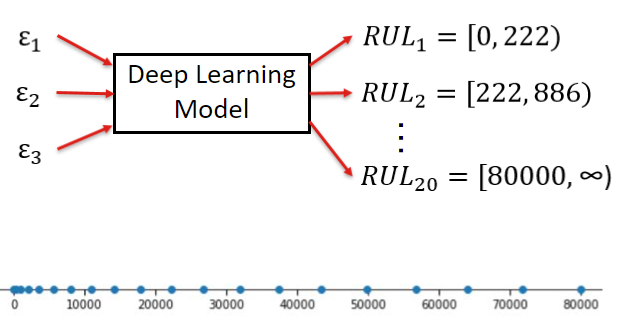
\includegraphics[width=6cm]{RUL_Classification.png}
	\caption{\gls{rul} classification strategy}
	\label{fig:RNN-classification}
\end{figure}


To prepare the data for the \gls{cnn} and \glspl{rnn} models a sliding window approach was used. This approach maps the \gls{rul} at time $ t_i $ onto the current and past time steps of the input features $ [x_{t-N+1}, x_{t-N+2},..., x_{t-1}, x_t] $ where $ N $ is the length of the sequence. The resulting input matrix therefore has the dimension $ k \times N $ where $ k $ is the number of features.

As an input for the different models, datasets had to be normalized. While a specific layer was added at the beggining of \gls{cnn} and \gls{tcn} architectures to do so, the preprocessed data had to be normalized before being fed to the \glspl{rnn} models.

% Add details on the explanation of the RNN Deep Learning models (Thomas)

\noindent
\textbf{Recurrent Neural Networks}

The common type of Deep Learning model for time series prediction are \glspl{rnn} \cite{Bai2018}. Due to their ability to store information within the cell, it can better remember information of a time-dependant data. 


\begin{figure}[htp]
	\centering
	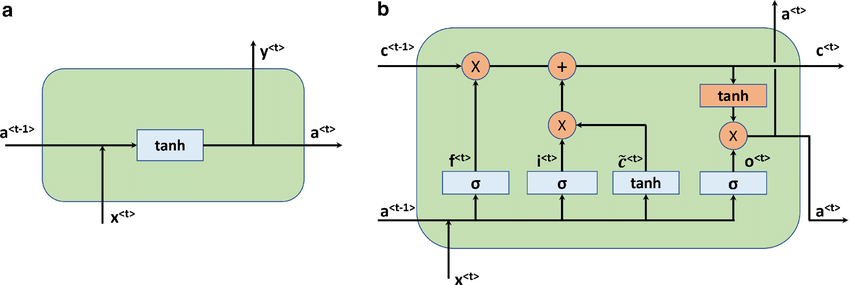
\includegraphics[width=6cm]{RNN-cell-architecture.png}
	\caption{RNN cell architecture. a. A simple RNN unit; b. an LSTM unit \cite{Chen2021}}
	\label{fig:RNN-classification}
\end{figure}

However, standard \glspl{rnn} have some major drawbacks, such as the vanishing or exploding gradient problem, which limit their application \cite{Bengio1994}. \gls{lstm} networks (Hochreiter and Schmidhuber \cite{Hochreiter1997}) avoid this problem and have established themselves as one of the most used Deep Learning model types, especially for \gls{nlp} \cite{Wu2016}. For these reasons \glspl{lstm} will be one of the investigated \gls{rnn} approaches in this project. Another investigated \gls{rnn} approach is the \glspl{gru}. It is a simplified version of the \gls{lstm}. Due to this simplicity it has been gaining in popularity in recent years \cite{Rana2016}. 

The key idea to \gls{gru} and \gls{lstm} is the memory cell which allows the network to remember information without much loss.

\gls{lstm} architecture consists in an input gate, a forget gate and an output gate. The input gate decides to add new information from the present input to the present cell state scaled by how much it wishes to add them. The forget gate allows the cell to know how to partially forget the previous cell state. Then, the output gate decides what to output from the new celle state.

For the \gls{gru} architecture, only two gates are implemented. The update gate decides the portion of updated candidate needed to calculate the current cell state, which in turn also decides the portion of the previous cell state retained. The relevance gate calculates how relevant the previous information is, and then is used in the candidate for the updated value.

Then, a simple \gls{rnn} architecture will be explored to evaluate the possible benefits of more complex structures. An \gls{rnn} unit only have a tanh layer after combining the cell state and the candidate.






% Add details on the explenation of the CNN Deep Learning models (Paul)

\noindent
\textbf{Convolutional Neural Networks}

Recent results suggest that \glspl{cnn} can match or even outperform \glspl{rnn} in time series related tasks \cite{Bai2018}. The second major focus of this work are therefore \gls{cnn} models.

The common \gls{cnn} models deal with 2-Dimensional data as input such as pictures. The time sequence data used for \gls{phm} is in 1-Dimensional format. For this application 1D-\gls{cnn} have been introduced. The key differences between them and the 2D-\glspl{cnn} are that their input data is reduced by one dimension and the convolution filter only slides in one dimension \cite{Akrim2021}. Figure \ref{fig:1D_cnn_architecture} shows an example of a simple \gls{cnn} architecture with an illustration of the filter sliding over the time series. 

\begin{figure}[htp]
	\centering
	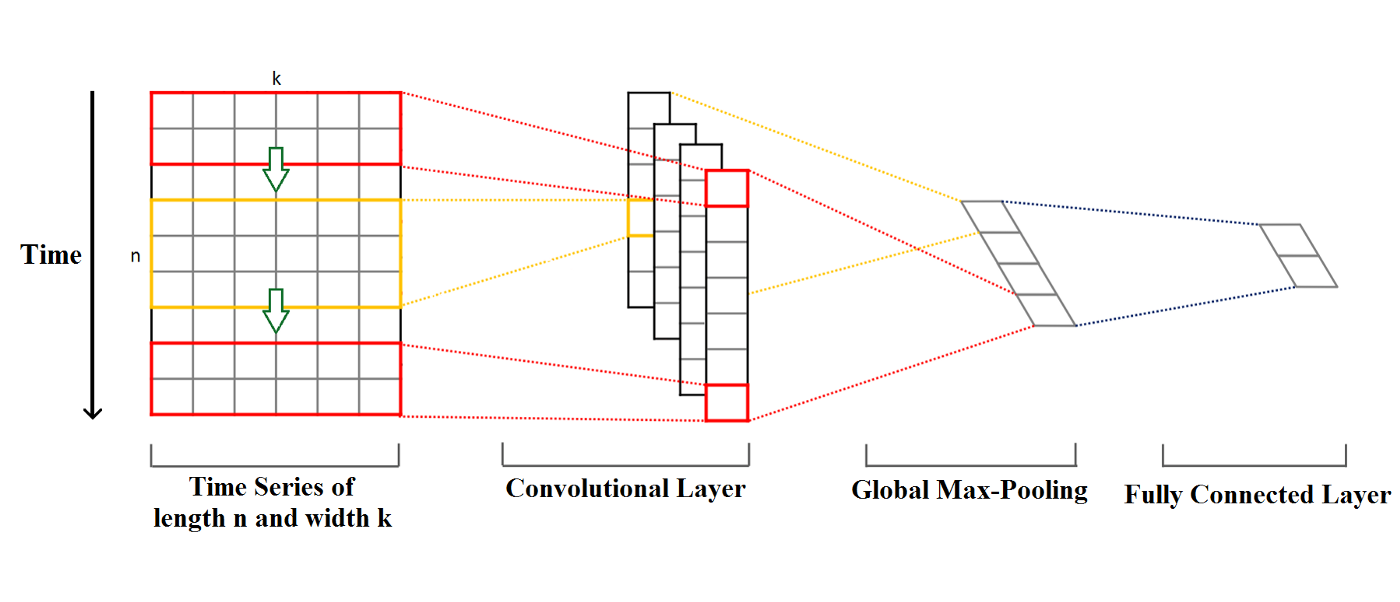
\includegraphics[width=0.5\textwidth]{1D_CNN_Architecture.png}
	\caption{Example of an 1D-\gls{cnn} architecture \cite{Sayyad}}
	\label{fig:1D_cnn_architecture}
\end{figure}

Besides the general \gls{cnn} architectures \glspl{tcn} (Bai et al. \cite{Bai2018}) are investigated in this work. A \gls{tcn} is a specific \gls{cnn} architecture that tries to replicate some of the best practices for \gls{cnn} architectures. As depicted in Fig. \ref{fig:tcn_architecture} a \gls{tcn} is composed of multiple layers which include dilation. The dilation for each layer can be set arbitrary but it is common practice to use multiples of $ 2 $ for it. Through dilation \glspl{tcn} can increase their receptive field and therefore capture relationships over longer time sequences. One \gls{tcn} layer is composed of a \gls{tcn} residual block (see Figure \ref{fig:tcn_block} (a)). One block consists of two dilated convolutional layers. The activation function for the layers is always the ReLu function. The residual blocks include dropout and normalization layers between the convolutional layers. The blocks also include an optional skip connection with a 1x1 convolutional layer. Figure \ref{fig:tcn_block} (b) shows an exemplary \gls{tcn} block with a kernel size of $ k = 3 $ and a dilation of $ d = 1 $. For more details on \glspl{tcn} see \cite{Bai2018}.

\begin{figure}[htp]
	\centering
	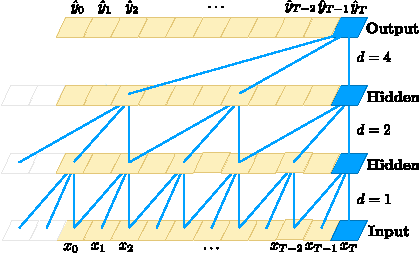
\includegraphics[width=7cm]{tcn_architecture.pdf}
	\caption{\gls{tcn} with dilation factors d = 1; 2; 4 and filter size k = 3 \cite{Bai2018}}
	\label{fig:tcn_architecture}
\end{figure}

\begin{figure}[htp]
	\centering
	\subfloat[][]{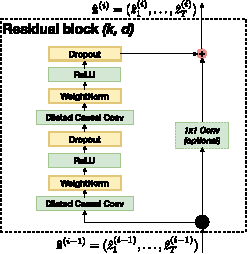
\includegraphics[width=0.2\textwidth]{tcn_block.pdf}}
	\qquad
	\subfloat[][]{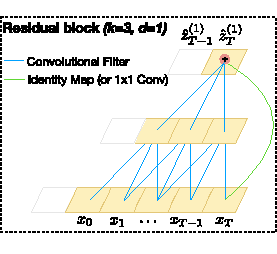
\includegraphics[width=0.2\textwidth]{tcn_block_example.pdf}}
	\caption{\gls{tcn} block elements, (a): Generic \gls{tcn} block, (b): Example for a \gls{tcn} block \cite{Bai2018}}
	\label{fig:tcn_block}
\end{figure}

% Maybe list the used frameworks (Keras, Tensoflow etc.)(Paul)

\noindent
\textbf{Metric and loss function}

To evaluate the performance of developed models a metric is needed. As the networks are used to perform classification instead of regression the accuracy metric is used. This metric calculates how many of the predictions made with the dataset are correct (e.g. the right \gls{rul} range is predicted)

\begin{equation}
	\label{eq:categorical-cross-entrophy}
	Accuracy = \frac{Number \: of \: correct \: predictions}{Total \: number \: of \: predictions}.
\end{equation}

This metric is applied during training and validation to compare different models against each other. The final assessment of the models is made by applying the accuracy metric to the testing dataset.

The used loss function which is used as the objective function for minimization by the backpropagation algorithm is the categorical crossentrophy loss function

\begin{equation}
	\label{eq:categorical-cross-entrophy}
	CE = -log(\frac{e^{s_p}}{\sum_{j}^{C} e^{s_j}})	
\end{equation}

where $ s_j $ is the output of the network for Class $ j $ with $ s_p $ beeing the positive class.

% Details on the hyperparameter optimization strategies (how the models are trained and how their parameters are optimised) (Paul)

\noindent
\textbf{Hyperparameter Optimization}

To optimize the proposed network architectures a hyperparameter optimization is performed. The hyperparameters include the parameters for the training process (Learning rate and batch size), network parameters (Dropout rate, activation funciton etc.) and the network architecture itself (number of layers, size of the layers etc.).

There are different strategies for hyperparameter optimization which can be divided in Model-Free and Model-Based approaches. For this study only Model-Free approaches are considered as they are more common and easier to apply. The two common approaches are grid search and random search \cite{Feurer2019}. 

For grid search the user defines a discrete number of values for each parameter. The algorithm then tries out all possible combinations of these sets of values. This quickly leads to an exesive amount of training runs that need to be done as the number of possible combinations $ B $ grows exponentially with the dimensionality $ d $ of the search space. If the number of values per parameter is $ n = 3 $ and the dimensionality is just $ d = 5 $ the number of combinations already equals $ B = n^d = 243 $.

Random search works with a fixed number of evaluations where for each evaluation a value randomly is selected from a predefined set of values for each parameter. The set of values can either be continuous with a lower and upper bound for the values or a discrete set of predefined values. Random search works better than grid search when some parameters are more important than others, which is a property that holds true in many cases \cite{Feurer2019}. Figure \ref{fig:grid_search_random_search} illustrates this property for one important and one unimportant parameter. With a fixed amount of $ B $ evaluations random search can evaluate up to $ B $ different values for each parameter. Whereas grid search is limited to $ B^{1/N} $ values per parameter. It is expected that the networks in this study behave like most networks with regard to the varying importance of the hyperparameters and therefore random search is choosen for hyperparameter optimization.

\begin{figure}[htp]
	\centering
	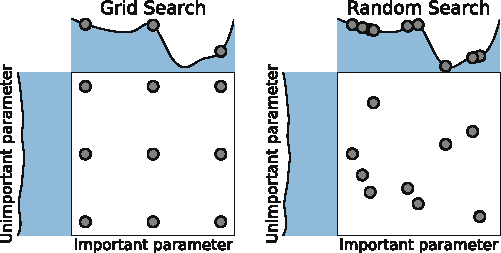
\includegraphics[width=7cm]{grid_search_random_search.pdf}
	\caption{Comparison of grid search and random search for an important and a unimportant parameter with 9 evaluations \cite{Feurer2019}}
	\label{fig:grid_search_random_search}
\end{figure}

To select the best model after performing the hyperparameter optimization the accuracy of the model on the validation dataset is used.

\noindent
\textbf{Fine Tuning}

After the optimum parameters for a model are found the model can be further improved by running more training epochs. To do so the models are trained with \gls{lrdecay)}. The best model from the hyperparameter optimization is taken and trained for a predefined number of epochs on the learning rate which was identified as the best one on the optimization. The learning rate is then lowered before the model is trained again for a fixed number of epochs. This step is repeated until convergence is achieved and no more significant improvements are visible. By using this approach the model in the early stages of training is less likely to get stuck in a local minimum and explores a wider range of possible configurations. As the training comes closer to an optimum the decaying learning rate helps with convergence and avoid oscillations. Besides this common beliefs there are probably more reasons to the effectiveness of \gls{lrdecay)}. According to You et al. \cite{You2019} is the initially large learning rate preventing the network from memorizing noisy data while the decaying learnig rate helps with learning complex patterns in the dataset.


\section{Results}
\label{sec:results}

% Show the used model architectures for rnn and cnn and why they are used (Paul and Thomas)

\noindent
\textbf{Model architectures}

Based on the \gls{cnn} architecture of Li et al. \cite{Li2018} which was used for aero-engine \gls{rul} prediction a vanilla \gls{cnn} architecture is generated. The first layer of the architecture is for layer normalization. Afterwards a flexible number of 1D-convolutional layers is added which all have the same number of filters and an identical kernel size. The output of the convolutional layers is flattend before the final dense output layer which has $ 20 $ nodes to match the number of \gls{rul} classes $ C = 20 $. As an example Figure \ref{fig:cnn_architecture_1000_structures} shows the final architecture after the hyperparameter optimization with 1000 training structures.

\begin{figure}[htp]
	\centering
	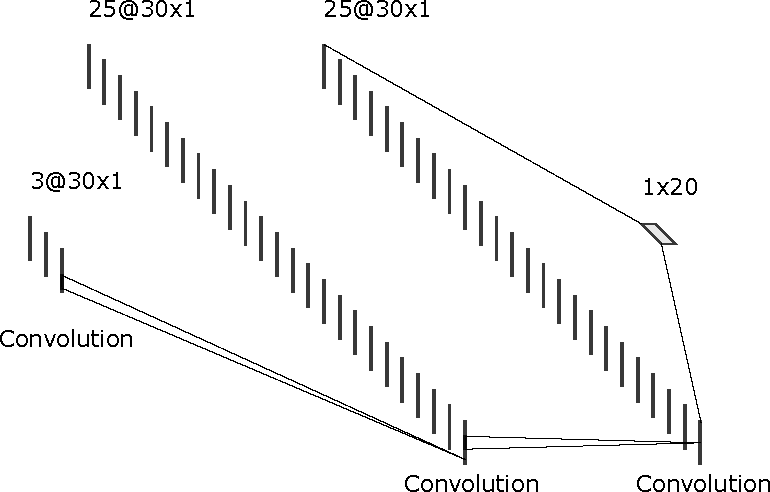
\includegraphics[width=0.5\textwidth]{cnn_architecture_1000_structures.pdf}
	\caption{\gls{cnn} architecture after hyperparameter optimization with 1000 training structures}
	\label{fig:cnn_architecture_1000_structures}
\end{figure}

A \gls{tcn} architecture template is generated based on the results of Liu et al. \cite{Liu2019} who used the network for \gls{rul} prediction of roller bearings. The architecture consists of multiple \gls{tcn} residual blocks with a dilation increasing with multiples of 2 with the first layer having a dilation of $ d = 1 $. Each block features the same number of filters with an identical kernel size. The next layer after the \gls{tcn} blocks is the dense output layer which has $ 20 $ nodes to match the number of \gls{rul} classes $ C = 20 $. The skip connection layer is activated for all residual blocks.

All \glspl{rnn} architectures were based on the same template. The dataset being noramlized before being fed to the models, there were no need for a specific layer of normalization. A flexible number of layers were implemented in the networks, from 1 hidden layer to a maximum of 3. Each layer includes from 32 to 256 units using a scaling by power of 2. A possible dropout and recurrent dropout could also be added for each layer, with a possibility of 0\% or 10\% for each. At the end of the architecture, a dense layer with 20 units were added in order to match the number of \gls{rul} classes $ C = 20 $.  

% Give an overview of the results of the hyperparameter optimisation strategies for the rnn and cnn networks (Paul and Thomas)

\noindent
\textbf{Hyperparameter optimisation}



% Show the detailed results of the fine tuning of some networks (Paul and Thomas)

% Compare the rnn and cnn results (Paul and Thomas)

\section{Conclusions}
\label{sec:conclusions}

% Give an overview of the general results of the study

% List the results of the best models and justify the choice for a best model

% Compare the final results with the aims set at the beginning

% Give an outlook for future research on the topic


\newpage
\printbibliography

\end{document}


